\documentclass{beamer}
\usepackage[utf8]{inputenc} %Input encoding
\usetheme{KUL}

\usepackage{amsmath} %Extra math symbols and operators
\usepackage{amssymb}
\usepackage{amsthm}
\usepackage{xcolor}
\definecolor{mygray}{gray}{0.95}

\usepackage{bm} %Bold symbols

\usepackage{graphicx} %Images
\usepackage{times}
%\addbibresource{../report/references.bib}
%\tikzset{component/.style={draw,thick,circle,fill=white,minimum size =0.75cm,inner sep=0pt}}
%\renewcommand{\thefigure}{\arabic{section}.\arabic{figure}}


\title{Presentation Bachelor Project}
\author{\phantom{=}Micha\"el Maex \and Rune Buckinx }
\date{March 2020}

\begin{document}
\maketitle
\begin{frame}{Introduction} %Bij deze slide gewoon korte intro geven over het project
    \huge{Modelling of Magnetohydrodynamic Waves in the Solar Corona}\\
    \Large{Ondertitel indien nodig}
\end{frame}

\begin{frame}
	\begin{enumerate}
		\item theorie
			\begin{enumerate}
				\item Niet wiskundige inleiding tot probleem
				\item bespreking vlg van HD en MHD
				\item afleiding dispersie relatie (heel kort)
				\item bespreking verschillende soorten golven
					\begin{itemize}
						\item Alfv\'en
						\item accoustic
					\end{itemize}
				\item fase en groepssnelheden (diagrammen)
			\end{enumerate}
		\item Pluto
			\begin{itemize}
				\item general info
				\item blastwave
			\end{itemize}
		\item MHD blastwave
		\item large scale structures
			\begin{itemize}
				\item hole
					\begin{itemize}
						\item reflectie coefficient
						\item vergelijking met observatie
					\end{itemize}
				\item plume
					\begin{itemize}
						\item reflectie in plume 
					\end{itemize}
			\end{itemize}
	\end{enumerate}
\end{frame}
\begin{frame}{Table of contents}
    \tableofcontents
\end{frame}
\section{Theory of MHD waves}
\begin{frame}{MHD Description of the Solar Corona}
    \centering
    Assumptions
    \begin{itemize}
        \item High collisionality
        \item Large Scale
        \item Ideal Fluid
    \end{itemize}
\end{frame}
\begin{frame}{HD Equations}
Euler equations for ideal fluids
\begin{alignat*}{4}
	&\text{Mass:} &\quad\quad &\frac{\partial \rho}{\partial t} & &+ \rho \nabla \cdot \mathbf v & &=  0 \\
	&\text{Momentum:} & \rho& \frac{\partial \mathbf v}{\partial t} & &+ \nabla p & &= 0\\
	&\text{Energy/adiabatic equation:} & &\frac{\partial }{\partial t} \left( \frac{p}{\rho^{\gamma}} \right)  & & & &= 0
\end{alignat*}
\end{frame}
\begin{frame}{MHD Equations}
    \begin{alignat*}{4}
	&\text{Mass:} &\quad\quad &\frac{\partial \rho}{\partial t} & & +\rho \nabla \cdot \mathbf v& &= 0 \\ 	
	&\text{Moment:} & \rho& \frac{\partial \mathbf v}{\partial t} & &+ \nabla p - \frac{(\nabla \times \mathbf B) \times \mathbf B}{\mu}& &=  0  \\
	&\text{Faraday's law:} & -&\frac{\partial \mathbf B}{\partial t} & &+ \nabla \times (\mathbf v \times \mathbf B)& &= 0 \\
	&\text{Energy:} & &\frac{\partial }{\partial t} \left( \frac{p}{\rho^{\gamma}} \right)  & & & &= 0 
\end{alignat*}
Magnetic pressure: $P_B = \frac{B^2}{2\mu}$. \\Plasma-$\beta$ : $\beta = \frac{p}{P_B} = \frac{2\mu}{B^2}$
\end{frame}

\begin{frame}{Dispersion Relation}
    Linearisation:
        \begin{equation*}
            f(\mathbf{x},t) = f_0(\mathbf{x}) + f_1(\mathbf{x},t)
        \end{equation*}
    Perturbations:
        \begin{equation*}
            \exp(i(\mathbf{kx} + \omega t))
        \end{equation*}
    Dispersion relation:
        \begin{equation*}
	        (\omega^2 - k^2 v_A^2 \cos^2 \theta)\left[ \omega^{4} - \omega^2k^2(v_A^2 + c_s^2) + k^{4}v_A^2c_s^2\cos^2\theta \right]  = 0
        \end{equation*}
        Where $c_s = \sqrt{\frac{\gamma p_0}{\rho_0}}$ and $v_A = \sqrt{\frac{\mathbf{B_0}^2}{\mu\rho_0}}$ and $\theta$
\end{frame}
\begin{frame}
    Dispersion relation:
        \begin{equation*}
	        (\omega^2 - k^2 v_A^2 \cos^2 \theta)\left[ \omega^{4} - \omega^2k^2(v_A^2 + c_s^2) + k^{4}v_A^2c_s^2\cos^2\theta \right]  = 0
        \end{equation*}
Three roots, three types of waves
\begin{align*}
&\text{1. Alv\'en waves:}	& \omega^2 &= k^2 v_a^2 \cos^2 \theta\\
&\text{Magneto accoustic waves:}\hspace{-4cm}\\
&\text{2. fast} 
& \omega^2 &= \frac{k^2}{2}\left( v_A^2 + c_s^2 + \sqrt{(v_a^2 + c_s^2) - 4 v_A^2 c_s^2 \cos^2\theta}  \right) \\
& \text{3. slow} & 
	\omega^2 &= \frac{k^2}{2}\left( v_A^2 + c_s^2 + \sqrt{(v_a^2 + c_s^2) - 4 v_A^2 c_s^2 \cos^2\theta}  \right) 
.\end{align*}
\end{frame}
\begin{frame}{Alfv\'en Waves}
	Assumptions: $\mathbf B_0 = B_0 \hat{x}$. 
	\begin{align*}
		\rho_0 \frac{\partial v_x}{\partial t}  - \frac{B_0}{\mu}\frac{\partial B_{1, x}}{\partial x}  &= 0 \\
		\frac{\partial B_{1,x}}{\partial t}  + B_0 \frac{\partial v_x}{\partial x} &= 0 
	.\end{align*}
	Interation between $B_x$ and $v_z$. 
	\begin{align*}
		\text{phase speed: } & \cos\theta \cdot v_A & \text{group speed: } & \pm v_A \cdot \hat{x}
	.\end{align*}
	\begin{itemize}
		\item Only move along magnetic field lines.
		\item Do not perturb density and pressure
	\end{itemize}
\end{frame}
\begin{frame}{Magnetosonic Waves}
	Interaction between density/pressure, velocity and magnetic field. 
	\begin{enumerate}
		\item slow waves:
			\begin{itemize}
				\item Move mostly among among field lines
				\item Predominantly visible when $\beta \gg 1$.
			\end{itemize}
		\item Fast waves:
			\begin{itemize}
				\item Move roughly isotropically 
				\item Predominantly visible when $\beta \ll 1$.
				\item Ordinary soundwaves when $\mathbf B = 0$
			\end{itemize}
	\end{enumerate}
\end{frame}
\begin{frame}
	\begin{figure}[h]
		\centering
		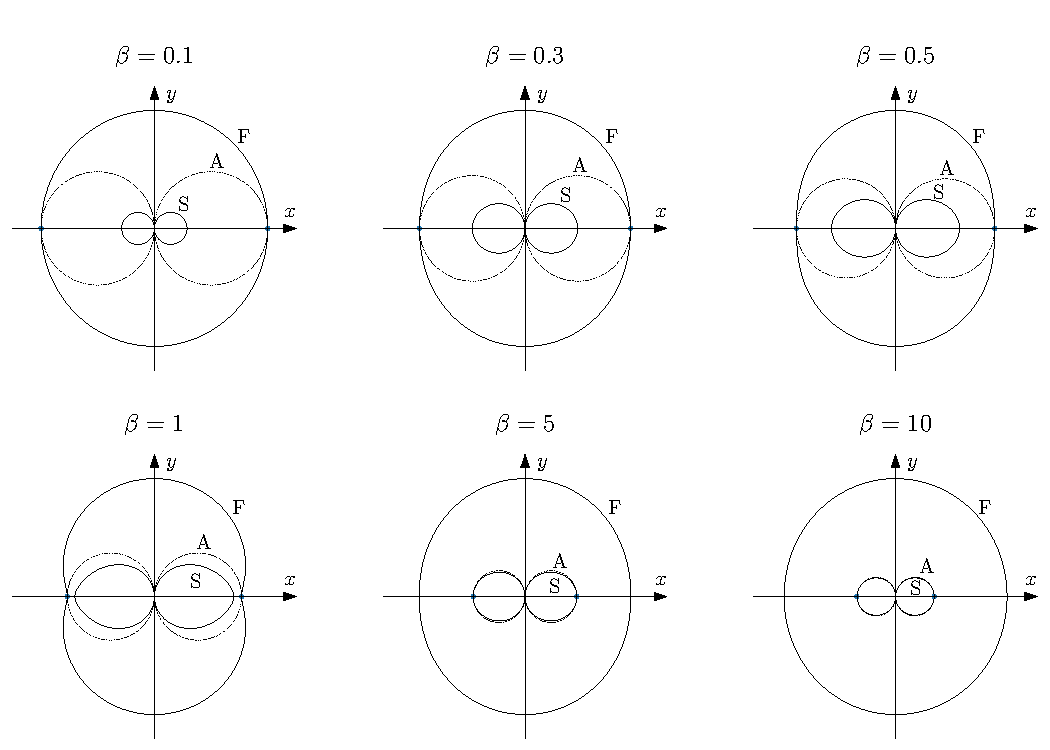
\includegraphics[width=0.8\textwidth]{../report/figures/fasespeed_beta.pdf}
		\caption{Phase speed for different $\beta$}	
	\end{figure}
\end{frame}
\begin{frame}
	\begin{figure}[h]
		\centering
		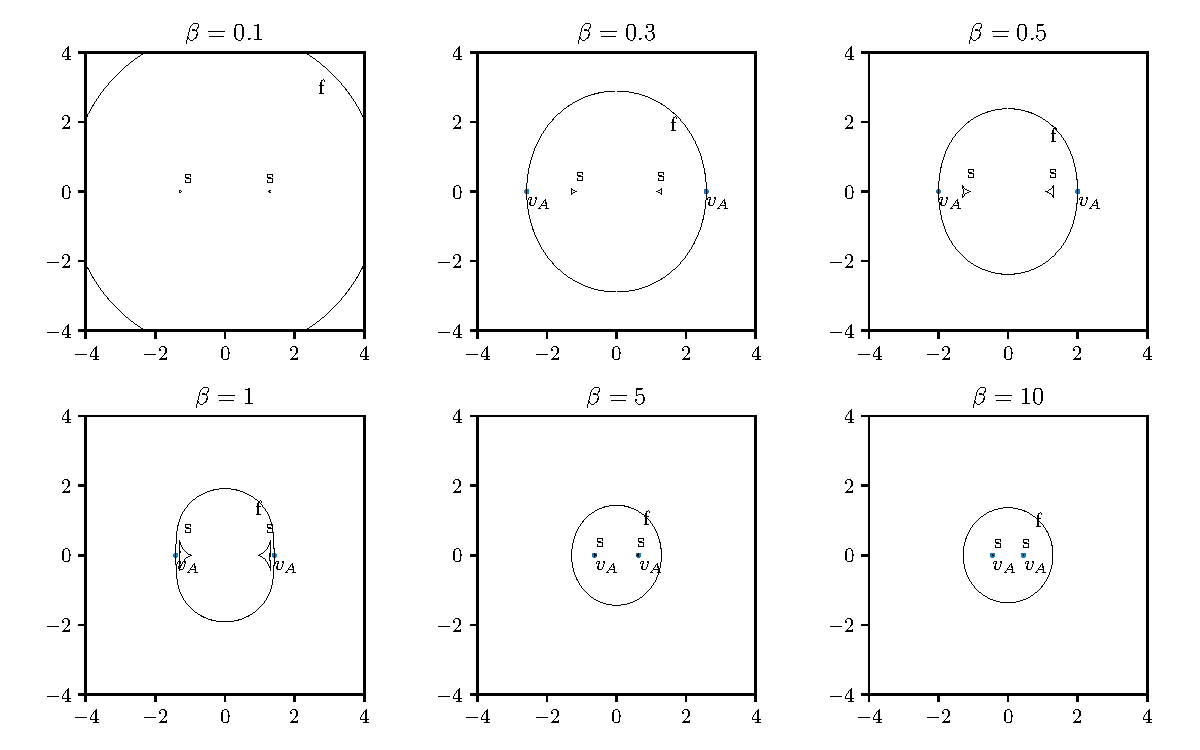
\includegraphics[width=.9\textwidth]{../report/figures/groupspeed_beta.pdf}
		\caption{Group speed for different $\beta$}
	\end{figure}	
\end{frame}

\section{PLUTO}
\begin{frame}{PLUTO}	
	The PLUTO Code for Astrophysical GasDynamics
	\begin{itemize}
		\item Uncompiled
			\begin{itemize}
				\item initial/boundary conditions needs to programmed in C.
				\item binary needs to be made for specific problem
			\end{itemize} 		\item Solvers for many equations (HD, MHD, relativisctic MHD, \ldots)
		\item Supports many types of geometry. 
	\end{itemize}
\end{frame}
\begin{frame}{Simple blastwave}

\end{frame}
\section{MHD Blastwave}
\begin{frame}{Frame Title}
    
\end{frame}
\section{Large Scale Structures}
\begin{frame}{Frame Title}
    
\end{frame}

\begin{frame}{References}
    \begin{itemize}\footnotesize{
        \item JP Hans Goedbloed and Stefaan Poedts. \textit{Principles of magnetohydrodynamics:with applications to laboratory and astrophysical plasmas.} Cambridge university press, 2004.
    }
    \end{itemize}
\end{frame}
\end{document}

